\documentclass[border=10pt]{standalone}

\usepackage{tikz}
\usepackage{tikzsymbols}
\usetikzlibrary{calc,patterns,shapes.geometric}

\def\centerarc[#1](#2)(#3:#4:#5){\draw[#1] ($(#2)+({#5*cos(#3)},{#5*sin(#3)})$) arc (#3:#4:#5);}

\begin{document}
	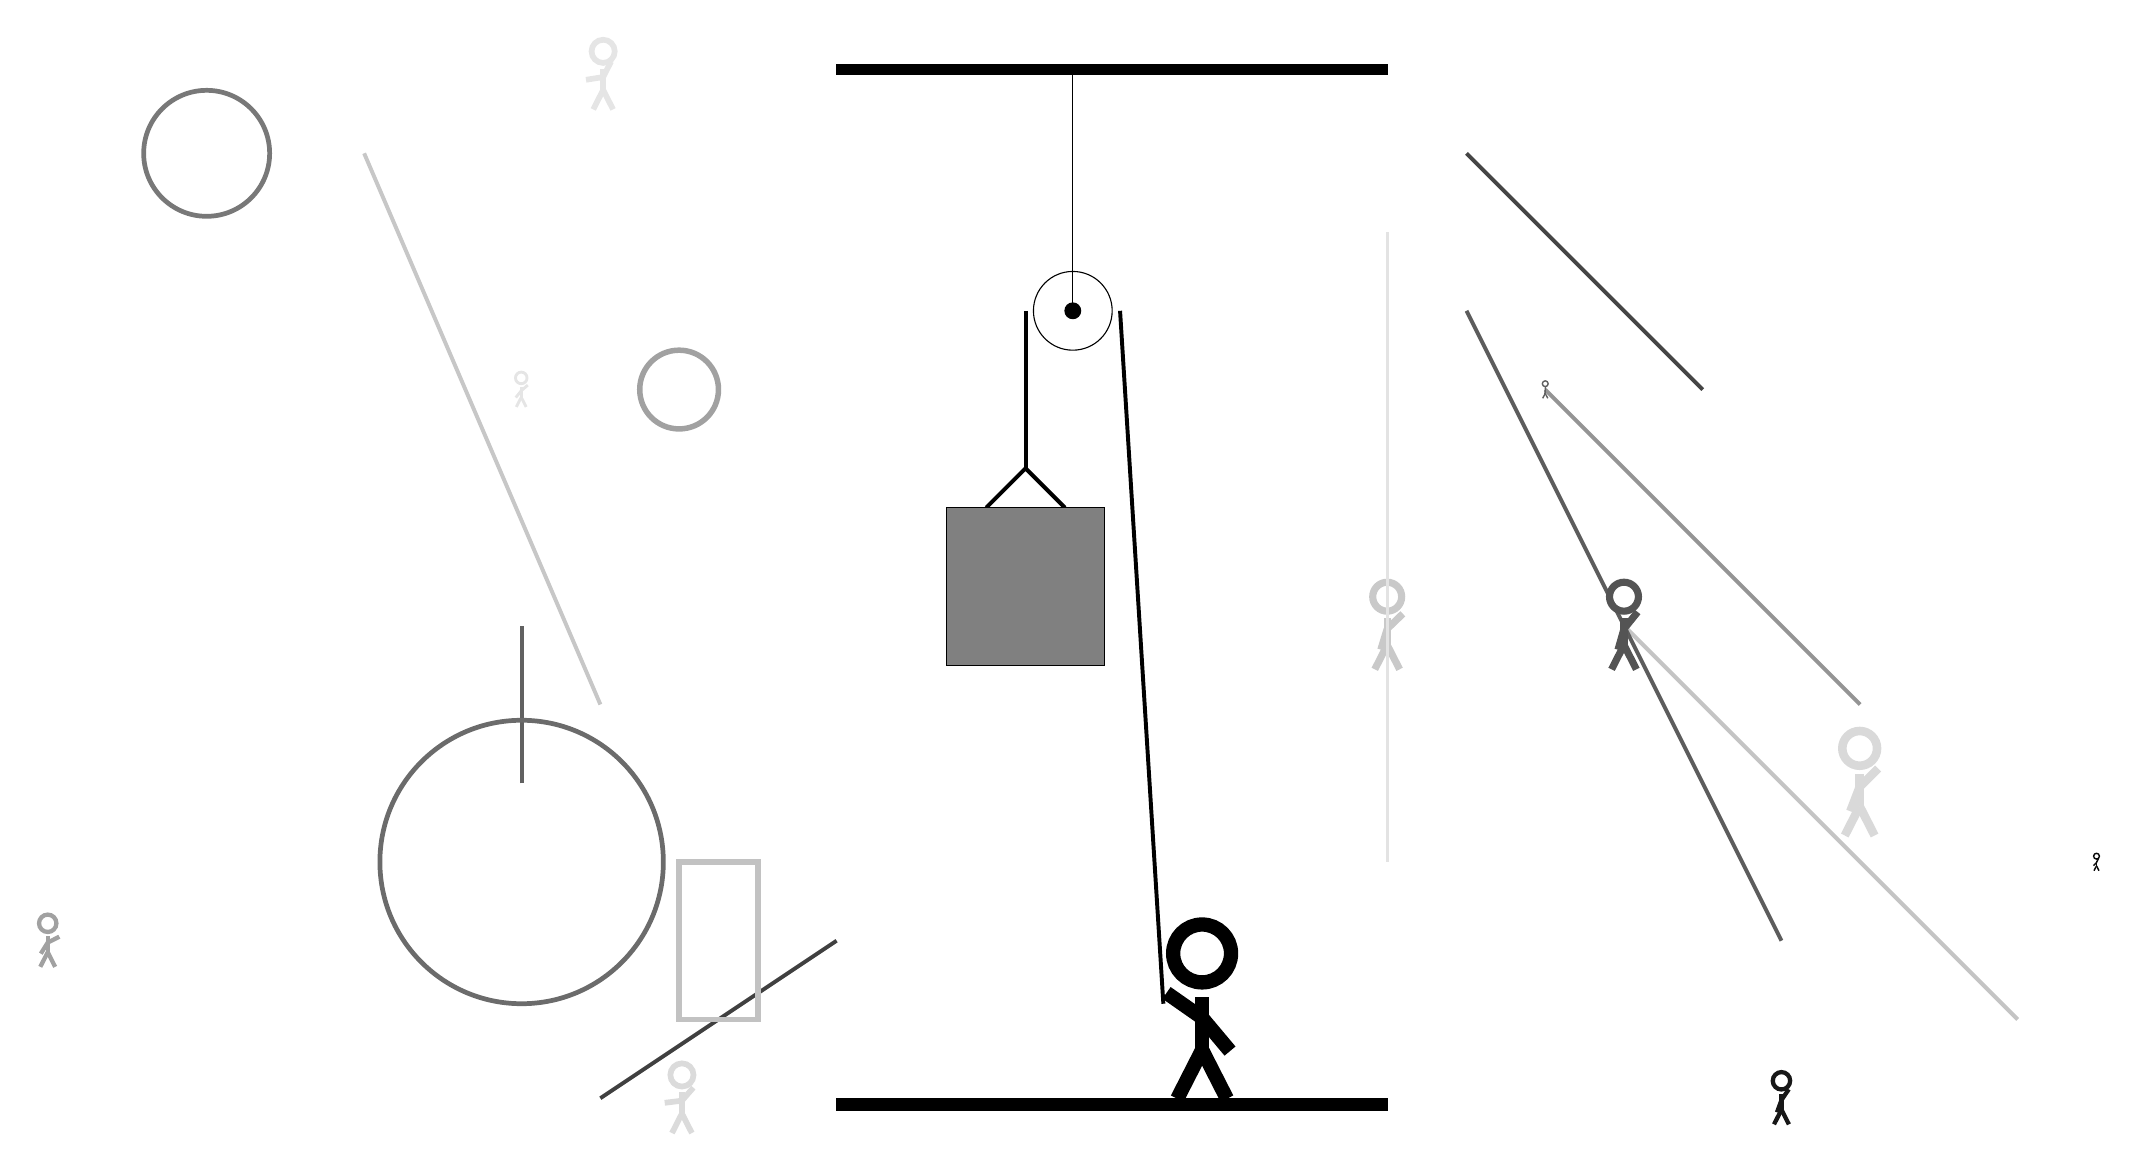
\begin{tikzpicture}
		%%%%% START %%%%%
		
		\draw[fill=black] (-2, 10) rectangle (5, 10.125);
		
		\draw (1, 7) circle (0.5);
		\draw[fill=black] (1, 7) circle (0.1);
		\draw (1, 10) -- (1, 7);
		
		\draw[line width=0.5mm] (-0.1, 4.5) -- (0.4, 5.0) -- (0.9, 4.5);
		\draw[fill=black!50] (-0.6, 4.5) rectangle (1.4, 2.5);
		
		\draw [line width=0.7mm, color=black!37](-4, 6) circle (0.5);
		
		\draw[line width=0.5mm, color=black!75](-5, -3) -- (-2, -1);
		\draw[line width=0.5mm, color=black!23](8, 3) -- (13, -2);
		\node[line width=0.7mm, color=black!10] at (-5, 10) {\Strichmaxerl[4][9][63]};
		
		\node[line width=0.3mm, color=black!10] at (-6, 6) {\Strichmaxerl[2][51][41]};
		\node[line width=0.2mm, color=black!21] at (5, 3) {\Strichmaxerl[5][73][44]};
		
		\draw[line width=0.5mm, color=black!42](7, 6) -- (11, 2);
		\draw[line width=0.5mm, color=black!73](6, 9) -- (9, 6);
		\node[line width=0.4mm, color=black!91] at (10, -3) {\Strichmaxerl[3][70][56]};
		
		\draw[line width=0.5mm, color=black!62](-6, 1) -- (-6, 3);
		\draw[line width=0.5mm, color=black!64](6, 7) -- (10, -1);
		\node[line width=0.5mm, color=black!15] at (11, 1) {\Strichmaxerl[6][69][45]};
		\draw [line width=0.6mm, color=black!53](-10, 9) circle (0.8);
		\node[line width=0.7mm, color=black!96] at (14, 0) {\Strichmaxerl[1][45][65]};
		\draw[line width=0.7mm, color=black!24] (-4, 0) rectangle (-3, -2);
		\draw[line width=0.5mm, color=black!22](-5, 2) -- (-8, 9);
		\node[line width=0.5mm, color=black!14] at (-4, -3) {\Strichmaxerl[4][7][49]};
		\draw [line width=0.6mm, color=black!58](-6, 0) circle (1.8);
		\node[line width=0.5mm, color=black!67] at (8, 3) {\Strichmaxerl[5][74][51]};
		\node[line width=0.4mm, color=black!62] at (7, 6) {\Strichmaxerl[1][84][85]};
		\node[line width=0.2mm, color=black!37] at (-12, -1) {\Strichmaxerl[3][58][27]};
		
		\draw[line width=0.4mm, color=black!11] (5, 0) rectangle (5, 8);
		
		\draw[line width=0.5mm] (0.4, 7) -- (0.4, 5.0);
		\centerarc[line width=0.5mm](1, 7)(0:180:0.6);
		\draw[line width=0.5mm](1.6, 7) -- (2.15, -1.8);
		
		\node at (2.6, -1.9) {\Strichmaxerl[10][-35][-50]};
		
		\draw[fill=black] (-2, -3) rectangle (5, -3.15);
		
		%%%%% END %%%%%
	\end{tikzpicture}
\end{document}